\documentclass[fleqn]{article}
\usepackage[T1]{fontenc}
\usepackage[utf8]{inputenc}
\usepackage{geometry}
\usepackage{graphicx}
\usepackage{url,hyperref}
\usepackage{xcolor,listings}
\usepackage{textcomp}
\usepackage{float}
\usepackage[bottom]{footmisc}
\usepackage{fancyvrb}
\usepackage{textcomp}
\usepackage{color}
\usepackage{footnote}
\usepackage{tabularx}
\usepackage[detect-all]{siunitx}
\sisetup{range-phrase = \text{--}}
\usepackage{commath}
\usepackage{adjustbox}
\usepackage{multirow}
\usepackage{amsmath}
\usepackage{amssymb}
\usepackage{enumerate}
\usepackage[shortlabels]{enumitem}
% \usepackage{subfig}
\usepackage{listings}
\usepackage[toc,page]{appendix}
% \usepackage[font={small},labelfont=bf]{caption}
\usepackage{subcaption}

\makesavenoteenv{table}

\hypersetup{
	colorlinks = true,
	citecolor = green,
	urlcolor = cyan
}

\definecolor{codegreen}{rgb}{0,0.6,0}
\definecolor{codegray}{rgb}{0.5,0.5,0.5}
\definecolor{codepurple}{HTML}{C42043}
\definecolor{backcolour}{HTML}{F2F2F2}
\definecolor{bookColor}{cmyk}{0,0,0,0.90}
\color{bookColor}

\newcommand{\xRightarrow}[2][]{\ext@arrow 0359\Rightarrowfill@{#1}{#2}}

\lstset{
	upquote=true,
	basicstyle=\ttfamily,
	columns=fullflexible,
	frame=single,
	breaklines=true,
	postbreak=\mbox{\textcolor{red}{$\hookrightarrow$}\space},
}

\lstdefinestyle{mystyle}{
	backgroundcolor=\color{backcolour},
	commentstyle=\color{codegreen},
	keywordstyle=\color{codepurple},
	numberstyle=\numberstyle,
	stringstyle=\color{codepurple},
	basicstyle=\footnotesize\ttfamily,
	breakatwhitespace=false,
	breaklines=true,
	captionpos=b,
	keepspaces=true,
	numbers=left,
	numbersep=10pt,
	showspaces=false,
	showstringspaces=false,
	showtabs=false,
}

\title{
	Topological Data Analysis \\
	Group project: \\
	Text 2
}
\author{
	Marko Prelevikj\\
	63130345\\
	\texttt{mp2638@student.uni-lj.si}
	\and
	Bozhidar Stevanovski\\
	63190410\\
	\texttt{bs9682@student.uni-lj.si}
}
\newcolumntype{m}{>{\hsize=.4\hsize}X}
\newcolumntype{s}{>{\hsize=.2\hsize}X}
\date{\today}

\begin{document}
	
	\maketitle
	\section{Introduction} \label{intro}
	% TODO: Bozhidar
	One of the earliest known literary works is \textit{Epic of Gilgamesh} dating from cca. 2150 BC. Today, after many centuries, the literature evolved and expanded, and now includes even a variety of literary genres. 
	
	Although the Sumerians/Babylonians did not live in a time when computers are available in order to write about the Gilgamesh's tale on one, today we have a lot of literary works in a digital format, enabling whole new fields which work with them, such as Natural Language Processing (NLP). One of the recent advances in the NLP field was due to the text embedding methods, which have shown to be able to effectively capture underlying semantic and syntactic information. 
	
	In this project we use persistence homology on sentence-level text embedding to explore differences in literary genres.
	
	
	\section{Methodology} \label{methods}
	Our method follows the basic principles of topological data analysis: picking a dataset, preprocessing it, building a complex, calculating homology, and finally evaluating the model. In the following subsections we explained each step a bit more granularly. We performed our experiment on a corpus of 1941 distinct text documents. We repeated our experiment twice: first including all words from the texts, and repeated with omitting all stop words.
	
	\subsection{Dataset} \label{dataset}
	There have been written a lot of literary works so far, and with the rise of the Internet, a lot of them have been made publicly available for anyone to access for free. One such online source is Project Gutenberg~\cite{projectGutenberg}, where each book has been classified in at least one category, or in their terms, a bookshelf. 
	
	For our purposes, we have used a preprocessed dataset by Lahiri~\cite{lahiri:2014:SRW}, which consists of more than 3000 text documents, each representing a single literary work. Each document is identified by the name of its author and its title. The downside of this dataset is that, unfortunately, it does not contain any information about the category to which the books belongs to.
	
	Finally, we categorized 37 authors into 8 distinct categories: \textit{mysticism}, \textit{historical}, \textit{children}, \textit{adventure}, \textit{psychological}, \textit{social}, \textit{detective} and \textit{plays}. The categorization was performed by determining the category of the majority of an author's books, for example majority of Sir Arthur Conan Doyle's books are detective because he was mostly writing about the adventures of Sherlock Holmes. The detailed categorization of each author and the amount of his/her documents used is presented in Appendix~\ref{app:dataset}.
	
	\subsection{Data processing} \label{preprocess}
	The pipeline for processing the data is rather simple: we split each document into its sentences and calculated the sentence embeddings using LASER~\cite{artetxe2018massively}. Each of the sentence embeddings contains 1024 components, so the result from LASER was a $1024\times N$, where $N$ is the number of sentences in the document. We squashed this matrix to a single column by averaging each component of the sentence embedding over all sentences, yielding a $1024\times1$ vector. We stack the resulting vectors into $1024\times M$ matrix, where $M$ is the number of documents for each category. Finally, we use \textit{SVD} decomposition to extract the first $r = 5$ components and reduce the final output to $5 \times M$, which we use for building our model of the data.
	
	For the second part of our experiment, we exclude all the stop words from the sentences. We perform the exclusion after dividing the document into sentences. To remove the stop words, we use \texttt{nltk}'s corpus~\cite{Loper02nltk:the} for English stop words.
	
	\subsection{Model} \label{model}
	% TODO: @Bozhidar
	% note: red dots are "redder" when there are more points at a single coordinate
	% Using the Gudhi library \cite{gudhi:urm}, 
	The reduced-dimension matrices are taken as input point clouds to produce an $\alpha$-shape complex. We have experimented with $2$ different approaches of selecting the increasing sequence of points for the filtration of our complex.
	
	The first (the naive and unsuccessful) one was selecting $R$ to be the largest distance between any two points in the point cloud, and taking the values $0=r_0 < r_1 < \dots < r_9 < r_{10} = R$ that partition the interval $[0,R]$ into $10$ equal parts to be the filtration values. However, since the $\alpha$-complex is a subcomplex of the $\check{C}$ech and the Delaunay, the value of $R$ turned out to be too large, and even the first sublevel complex using the value that one tenth as large as $R$, i.e. $r_1$, included all simplices of the $\alpha_\infty$ complex. Hence, this resulted in a trivial filtration: $S = K_{r_0} \leq K_{r_1} = \dots K_{r_{10}} = \alpha(S)$, where the point cloud is denoted with $S$. Therefore, this approach was discarded.
	
	In the second approach, after constructing the Delaunay complex ($\alpha_{\infty}$ complex), $R$ was chosen to be the largest radius of a k-simplex ($k \in \{0,1,2,3\}$) in it.  The filtration values $0=r_0 < r_1 < \dots < r_9 < r_{10} = R$ were again chosen by partitioning the interval $[0, R]$ into $10$ equal parts.
	
	
	Having the filtration of the $\alpha$ complex, we proceed to build the persistence diagrams for the first three dimensions of the data, i.e. for dimension $d \in \{0, 1, 2\}$. This procedure is identically repeated for each of the $8$ document type matrices, resulting in $8$ separate filtrations and their corresponding persistence diagrams.
	
	For the purposes of implementation we utilized the Gudhi library \cite{gudhi:urm}. However, since it works on the set of reals, we  discretized the birth and death values using our $r_i$ values. More specifically, each finite real value $v$ provided by Gudhi, was transformed as the smallest $r_i, i \in \{0, \dots, 10\}$ such that $r_i \geq r$. We should note that the case of such $r_i$ not to exist is impossible due to the way we chose $R = r_{10}$.
	
	Based on the persistence diagrams, we were able to calculate the pairwise bottleneck distances of each category, for all dimensions separately. We built a distance matrix $D$ with the obtained distances and we applied an agglomerative clustering algorithm in order to construct dendrograms.
	
	We chose to build dendrograms because they illustrate the hierarchical relationship of the underlying data. In our case we show the similarity of distinct literary categories, i.e. the most similar ones are connected first and then the most similar to the newly born category is merged, etc. until we have a single group consisting of all categories.
	
	The procedure was repeated two times, first taking all the words into consideration and including them in the embeddings, and a second repetition for the case when the stop-words are excluded. 
	
	\section{Results} \label{results}
	% As a result of the experiment we obtained two distinct sets of results. In both cases the model generated persistence diagrams for each category separately. The persistence diagram includes the first three dimensions of the data, i.e. $d \in \{0, 1, 2\}$, and are presented visually in Appendix~\ref{app:persistence}.
	
	As a result of the experiment we obtained two distinct sets of results, based on inclusion/exclusion of the stop words. In both cases the model generated persistence diagrams for each category separately, which are visually presented in Appendix~\ref{app:persistence}. They include the dimensions $0, 1$ and $2$ on same image, and the point multiplicity is handled by point-transparency, by including inversely proportional relationship between the multiplicity of a point and its transparency.
	The dendrograms we obtained from the bottleneck distances of the persistence diagrams are presented in Appendix~\ref{app:dendro}.
	
	The obtained dendrograms were closely examined by an experienced professional \footnote{Marko's mother is a high-school literature professor :)} and it was concluded that the dendrogram shown in Figure~\ref{fig:winner}, which is obtained by omitting the stop words and for $d = 0$ was an almost perfect classification from a semantic point of view of the categories. Even though the distances among the persistence diagrams for all categories are very small, the distinction between the categories and how the clusters are merged hierarchically together is correct.
	
	The rest of the dendrograms are performing rather worse. There are cases where the dendrograms do not make any sense, such a cases are presented in Figure~\ref{fig:all:d2} and Figure~\ref{fig:sw:d2}. But then again, there are also cases, such as in Figure~\ref{fig:all:d1}, where we observe that there is almost no distinction between the categories \textit{psychological} and \textit{detectives}, whilst \textit{historical}, \textit{children}, \textit{social} and \textit{adventure} are perfectly distinguished, just like in Figure~\ref{fig:winner}. This led us to the conclusion that there is a negative correlation between the dimension $d$ and the discriminatory performance of the persistence diagrams, i.e. with the increasing of the dimension, the performance is decreased. And thus, we concluded that we get the best performance in each case at $d = 0$.
	
	To achieve peak performance of our model we had to minimize the amount of noise we include in the input data, i.e. remove the stop words from the corpus which we used for analysis. Another indicator are the distances observed in both the persistence diagrams and the dendrograms, which are in the rank of $10^{-3}$, and when working with such small distances the probability of making an error is increased, since there is not much room left for error. Which led us to the conclusion that our model is very susceptible to noise.
	
	\begin{figure}
		\centering
		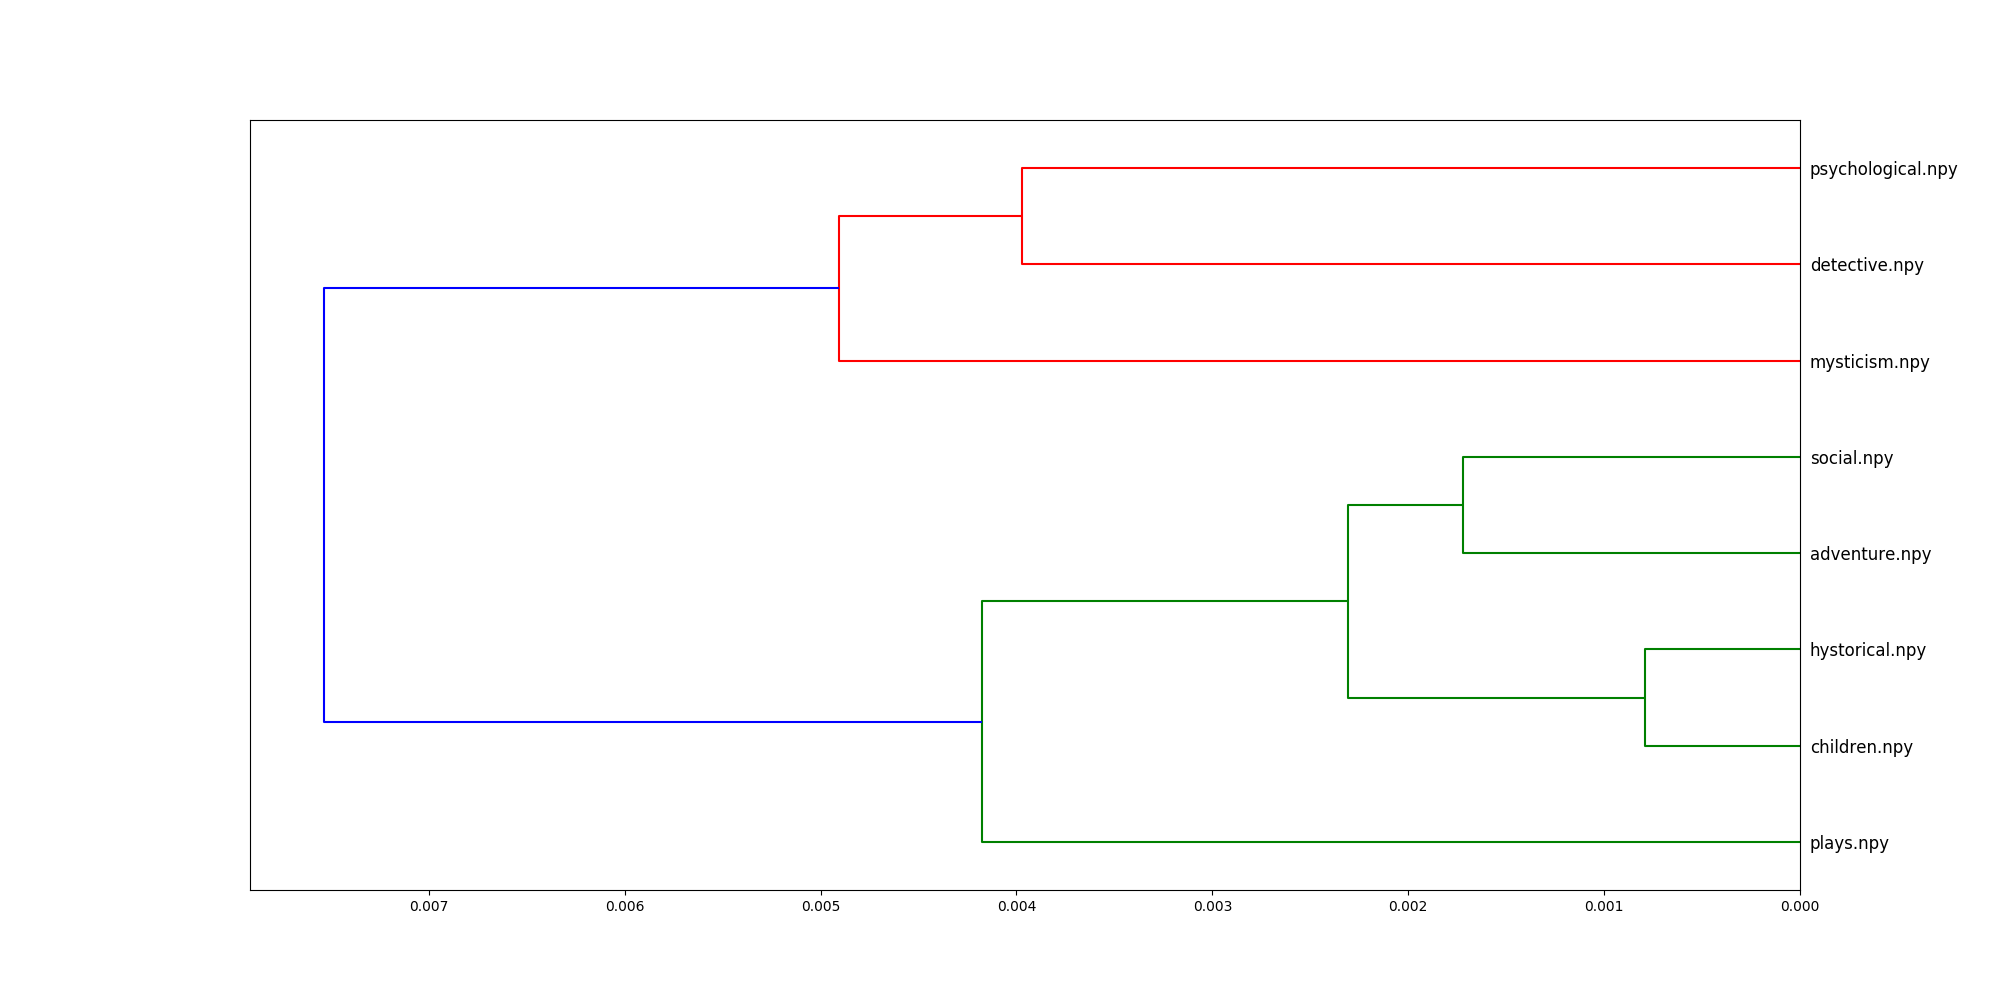
\includegraphics[width=0.9\textwidth]{figures/stopwords_excluded/dendrogram_d0.png}
		\caption{We obtained our experiment's best result by omitting the stop words at $d = 0$. The colours represent the discovered clusters, which merge together the most similar categories.}
		\label{fig:winner}
	\end{figure}
	
	\section{Conclusion} \label{conclusion}
	% TODO: Bozhidar
	In this project we presented an approach to capture the underlying semantic difference between literature categories, using persistence homology on sentence-level document embedding. We employ this model on eight categories (mysticism, historical, children, adventure, psychological, social, detective and plays). The evaluation showed that the persistence homology in dimension $0$ outperforms dimensions $1$ and $2$, and at this dimension, excluding the stop words from the documents yields perfect classification.
	
	\section*{Appendix} \label{appendix}
	\appendix
	\section{Dataset categorization} \label{app:dataset}
	The dataset categorization is presented in Table~\ref{tab:1}.
	
	\begin{table}[ht]
		\centering
		\begin{tabular}{r|l|r}
			Category & Author & Book count\\
			\hline
			\hline
			mysticism & William Wymark Jacobs & 97 \\
			& G K Chesterton & 39 \\
			& & $\sum = 136$ \\
			\hline
			historical & George Alfred Henty & 89 \\
			& William Dean Howells & 84 \\
			& Henry James & 72 \\
			& James Fenimore Cooper & 36 \\
			& Sir Walter Scott & 35 \\
			& William Makepeace Thackeray & 30 \\
			& & $\sum = 346$ \\
			\hline
			children & R M Ballantyne & 88 \\
			& Andrew Lang & 60 \\
			& Charlotte Mary Yonge & 60 \\
			& Jacob Abbott & 47 \\
			& Mark Twain & 47 \\
			& Charles Kingsley & 44 \\
			& Rudyard Kipling & 43 \\
			& Frank Richard Stockton & 32 \\
			& Thornton Waldo Burgess & 31 \\
			& & $\sum = 452$ \\
			\hline
			adventure & Robert Louis Stevenson & 79 \\
			& Bret Harte & 58 \\
			& Edward Stratemeyer & 58 \\
			& Henry Rider Haggard & 52 \\
			& Jack London & 48 \\
			& Harold Bindloss & 43 \\
			& Daniel Defoe & 40 \\
			& & $\sum = 378$ \\
			\hline
			psychological & Nathaniel Hawthorne & 86 \\
			& Joseph Conrad & 34 \\
			& & $\sum = 120$ \\
			\hline
			social & Anthony Trollope & 71 \\
			& Charles Dickens & 61 \\
			& John Galsworthy & 40 \\
			& P G Wodehouse & 35 \\
			& Louisa May Alcott & 34 \\
			& & $\sum = 241$ \\
			\hline
			detective & Sir Arthur Conan Doyle & 57 \\
			& Edward Phillips Oppenheim & 53 \\
			& Wilkie Collins & 32 \\
			& & $\sum = 142$ \\
			\hline
			plays & George Bernard Shaw & 42 \\
			& John Ruskin & 42 \\
			& Lyman Frank Baum & 42 \\
			& & $\sum = 126$ \\
		\end{tabular}
		\caption{Categorization of each author included in our experiment. The table lists how many of his/her works we included in our calculations and the sum of all documents per category. In total, we used 1941 distinct text documents.}
		\label{tab:1}
	\end{table}
	
	\section{Persistence diagrams} \label{app:persistence}
	The persistence diagrams of each categories are presented in Figure~\ref{fig:all} and Figure~\ref{fig:sw} for all words and with the omission of stop words, respectively.
	
	\begin{figure}
		\begin{subfigure}[t]{0.425\textwidth}
			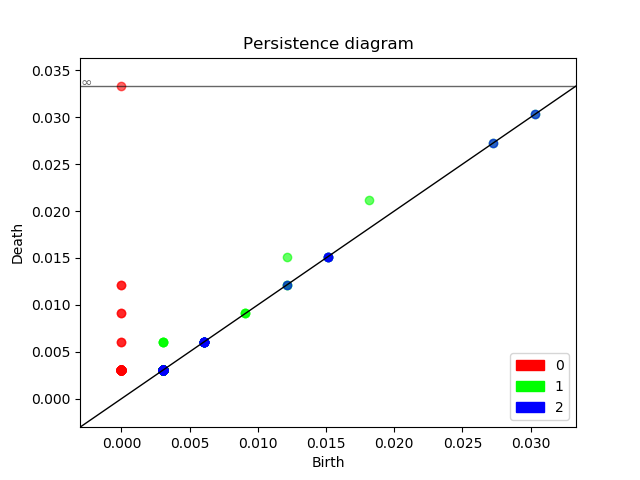
\includegraphics[width=\textwidth]{figures/all_words/mysticism.png}
			\caption{mysticism}
			\label{fig:all:mysticism}
		\end{subfigure}\hfill
		\begin{subfigure}[t]{0.425\textwidth}
			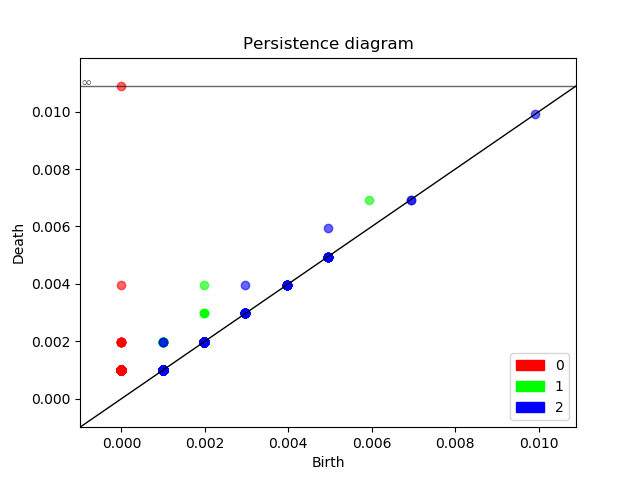
\includegraphics[width=\textwidth]{figures/all_words/hystorical.png}
			\caption{historical}
			\label{fig:all:historical}
		\end{subfigure}\hfill
		\\
		\begin{subfigure}[t]{0.425\textwidth}
			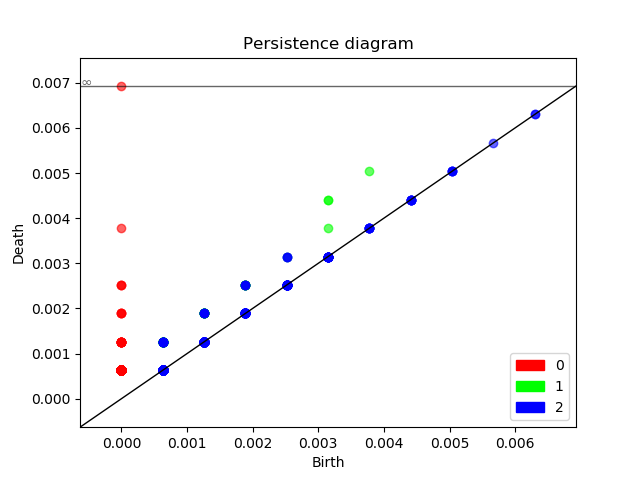
\includegraphics[width=\textwidth]{figures/all_words/children.png}
			\caption{children}
			\label{fig:all:children}
		\end{subfigure}\hfill
		\begin{subfigure}[t]{0.425\textwidth}
			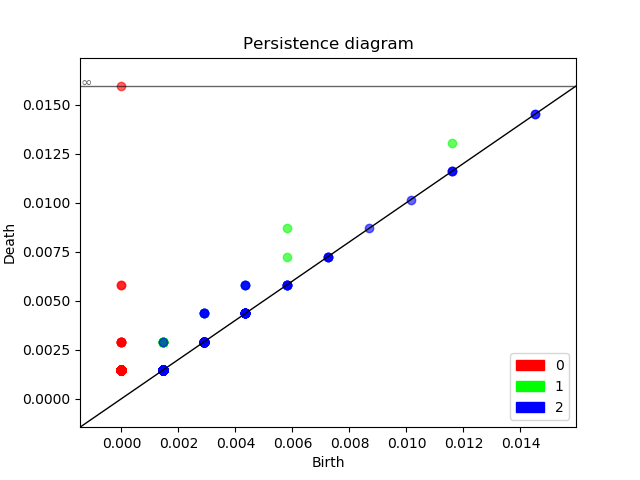
\includegraphics[width=\textwidth]{figures/all_words/adventure.png}
			\caption{adventure}
			\label{fig:all:adventure}
		\end{subfigure}\hfill
		\\
		\begin{subfigure}[t]{0.425\textwidth}
			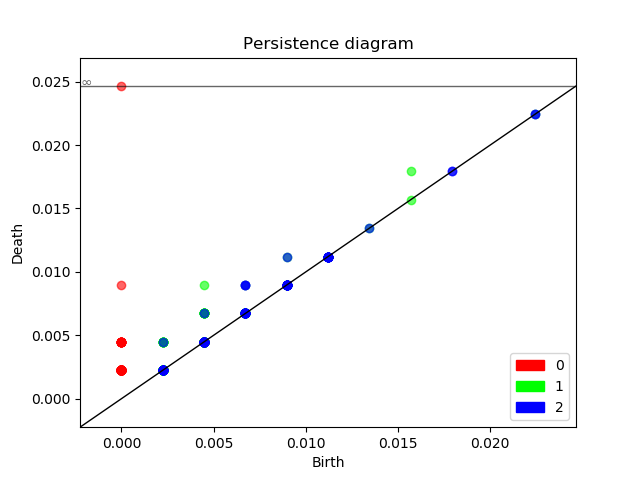
\includegraphics[width=\textwidth]{figures/all_words/psychological.png}
			\caption{psychological}
			\label{fig:all:psychological}
		\end{subfigure}\hfill
		\begin{subfigure}[t]{0.425\textwidth}
			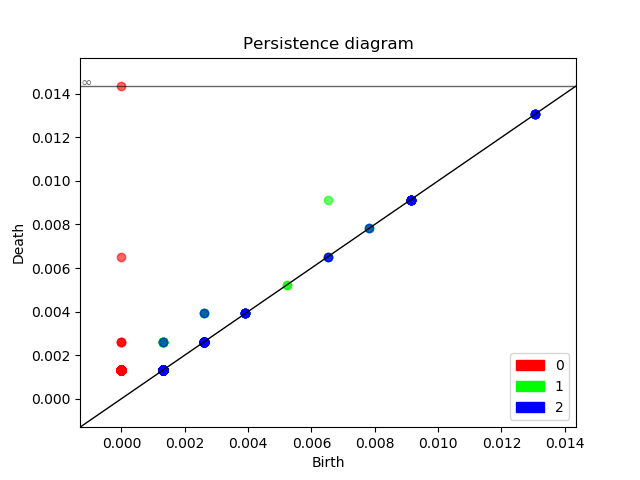
\includegraphics[width=\textwidth]{figures/all_words/social.png}
			\caption{social}
			\label{fig:all:social}
		\end{subfigure}\hfill
		\\
		\begin{subfigure}[t]{0.425\textwidth}
			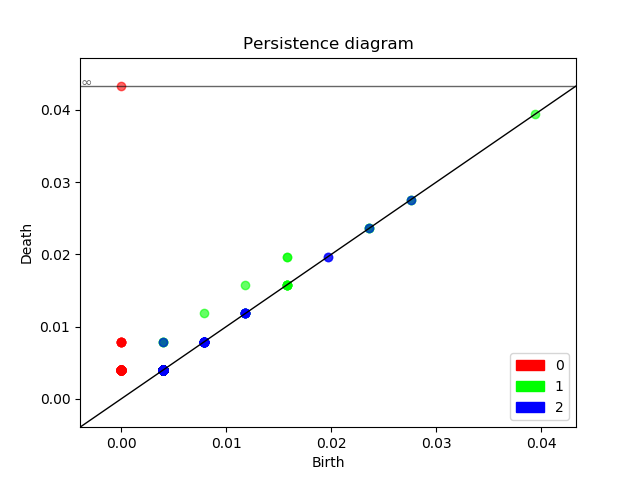
\includegraphics[width=\textwidth]{figures/all_words/detective.png}
			\caption{detective}
			\label{fig:all:detective}
		\end{subfigure}\hfill
		\begin{subfigure}[t]{0.425\textwidth}
			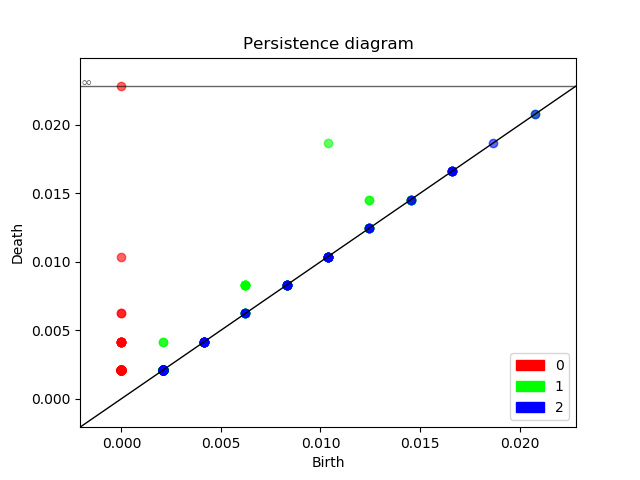
\includegraphics[width=\textwidth]{figures/all_words/plays.png}
			\caption{plays}
			\label{fig:all:plays}
		\end{subfigure}\hfill
		\caption{Persistence diagrams of documents per category including all words.}
		\label{fig:all}
	\end{figure}
	
	\begin{figure}
		\begin{subfigure}[t]{0.425\textwidth}
			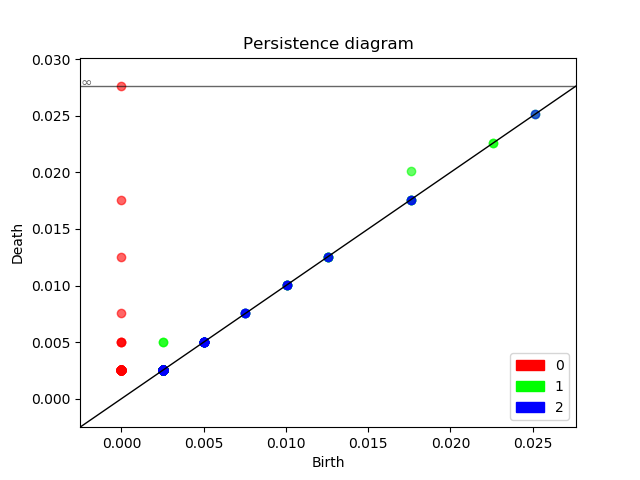
\includegraphics[width=\textwidth]{figures/stopwords_excluded/mysticism.png}
			\caption{mysticism}
			\label{fig:sw:mysticism}
		\end{subfigure}\hfill
		\begin{subfigure}[t]{0.425\textwidth}
			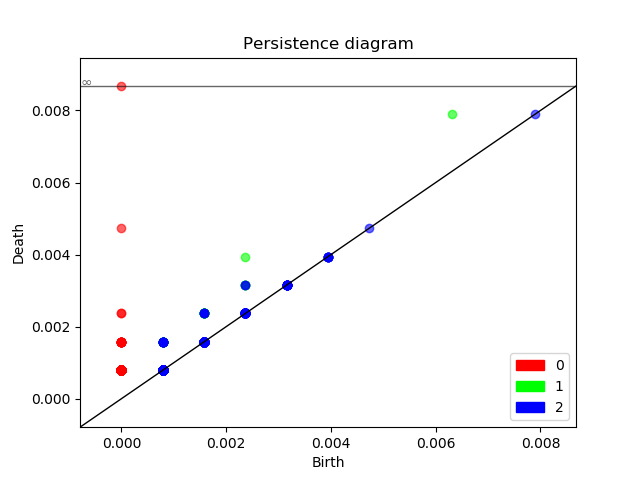
\includegraphics[width=\textwidth]{figures/stopwords_excluded/hystorical.png}
			\caption{historical}
			\label{fig:sw:historical}
		\end{subfigure}\hfill
		\\
		\begin{subfigure}[t]{0.425\textwidth}
			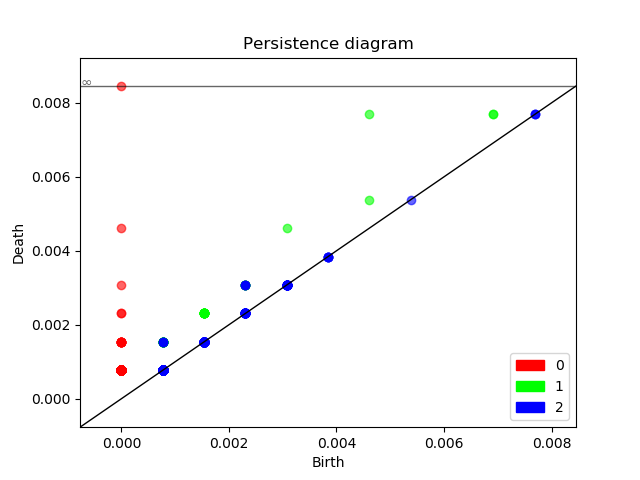
\includegraphics[width=\textwidth]{figures/stopwords_excluded/children.png}
			\caption{children}
			\label{fig:sw:children}
		\end{subfigure}\hfill
		\begin{subfigure}[t]{0.425\textwidth}
			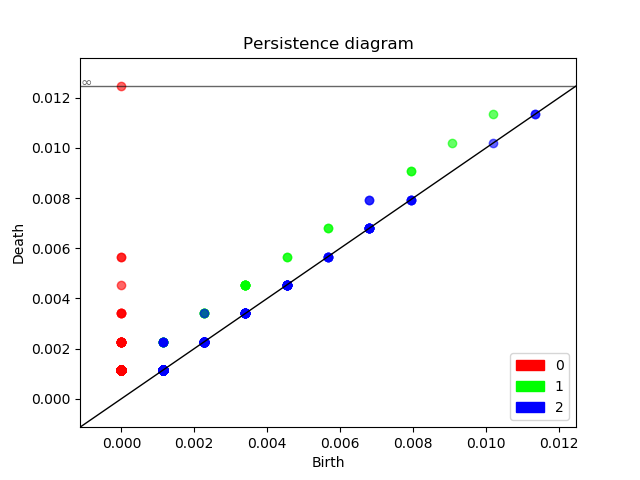
\includegraphics[width=\textwidth]{figures/stopwords_excluded/adventure.png}
			\caption{adventure}
			\label{fig:sw:adventure}
		\end{subfigure}\hfill
		\\
		\begin{subfigure}[t]{0.425\textwidth}
			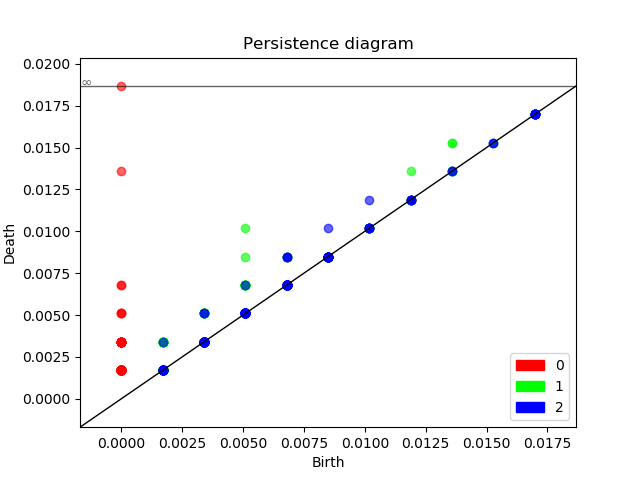
\includegraphics[width=\textwidth]{figures/stopwords_excluded/psychological.png}
			\caption{psychological}
			\label{fig:sw:psychological}
		\end{subfigure}\hfill
		\begin{subfigure}[t]{0.425\textwidth}
			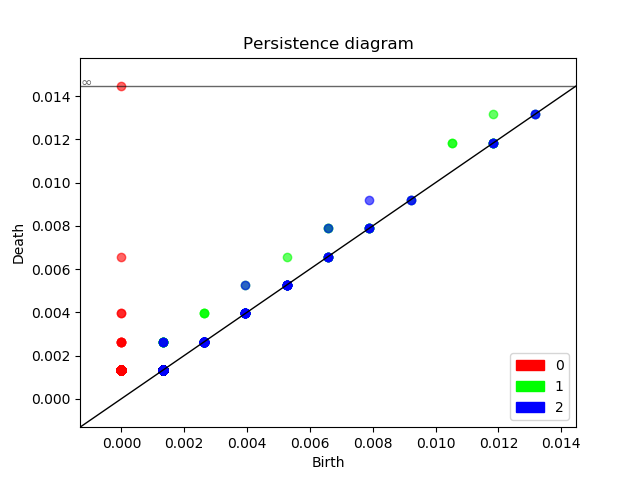
\includegraphics[width=\textwidth]{figures/stopwords_excluded/social.png}
			\caption{social}
			\label{fig:sw:social}
		\end{subfigure}\hfill
		\\
		\begin{subfigure}[t]{0.425\textwidth}
			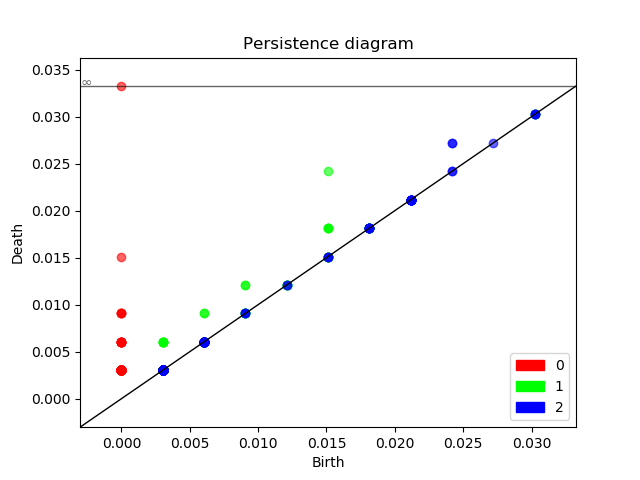
\includegraphics[width=\textwidth]{figures/stopwords_excluded/detective.png}
			\caption{detective}
			\label{fig:sw:detective}
		\end{subfigure}\hfill
		\begin{subfigure}[t]{0.425\textwidth}
			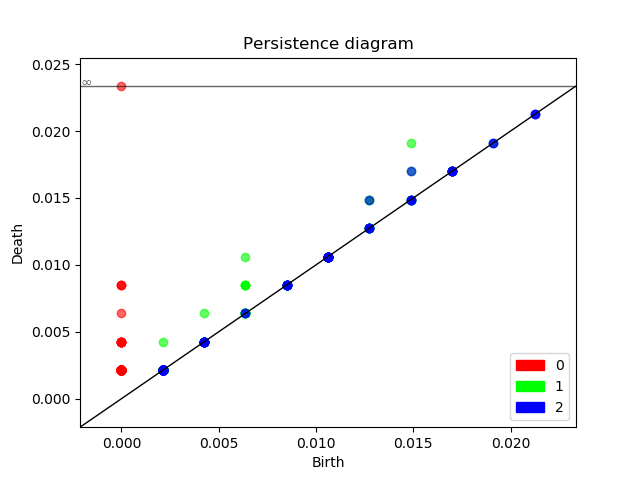
\includegraphics[width=\textwidth]{figures/stopwords_excluded/plays.png}
			\caption{plays}
			\label{fig:sw:plays}
		\end{subfigure}\hfill
		\caption{Persistence diagrams of documents per category omitting all stop words.}
		\label{fig:sw}
	\end{figure}
	
	\section{Dendrograms} \label{app:dendro}
	The resulting dendrograms from the distances among each persistence diagrams pairwise are presented in Figure~\ref{fig:dendro}.
	
	\begin{figure}
		\begin{subfigure}[t]{0.475\textwidth}
			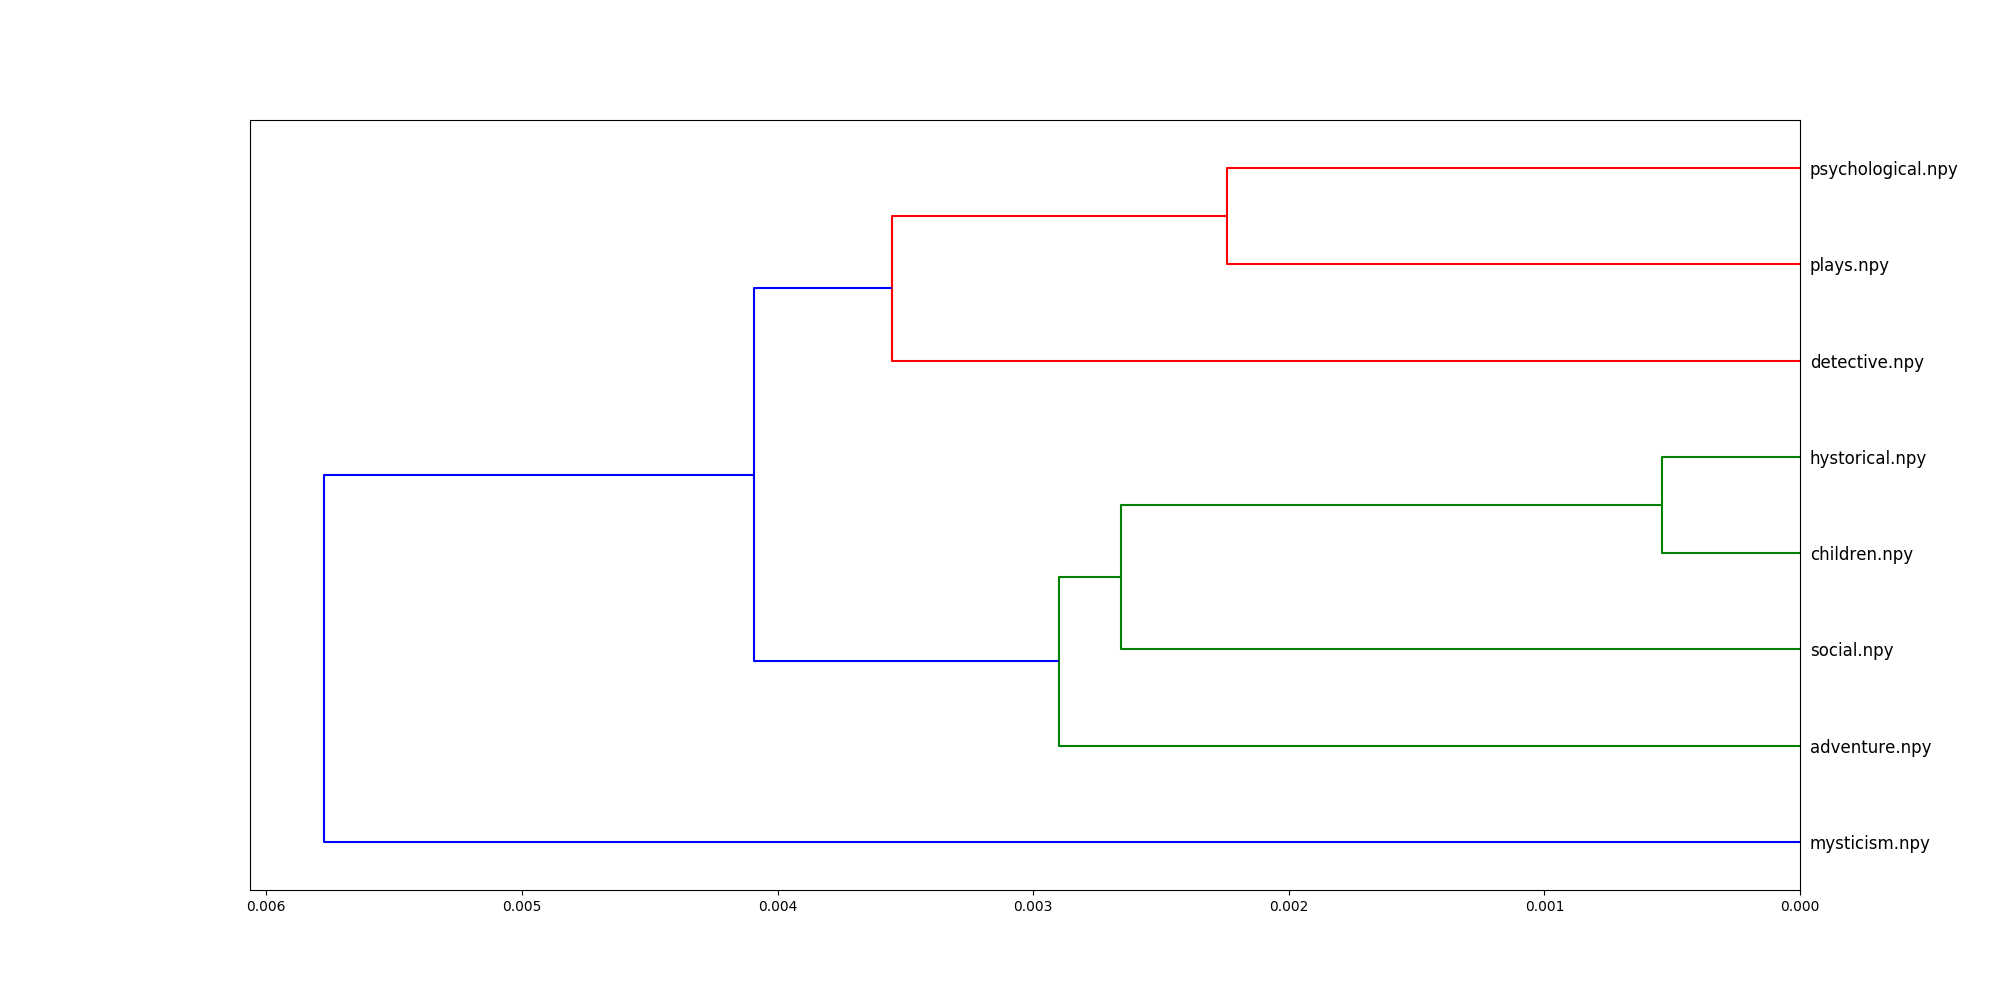
\includegraphics[width=\textwidth]{figures/all_words/dendrogram_d0.png}
			\caption{All words, $d = 0$}
			\label{fig:all:d0}
		\end{subfigure}\hfill
		\begin{subfigure}[t]{0.475\textwidth}
			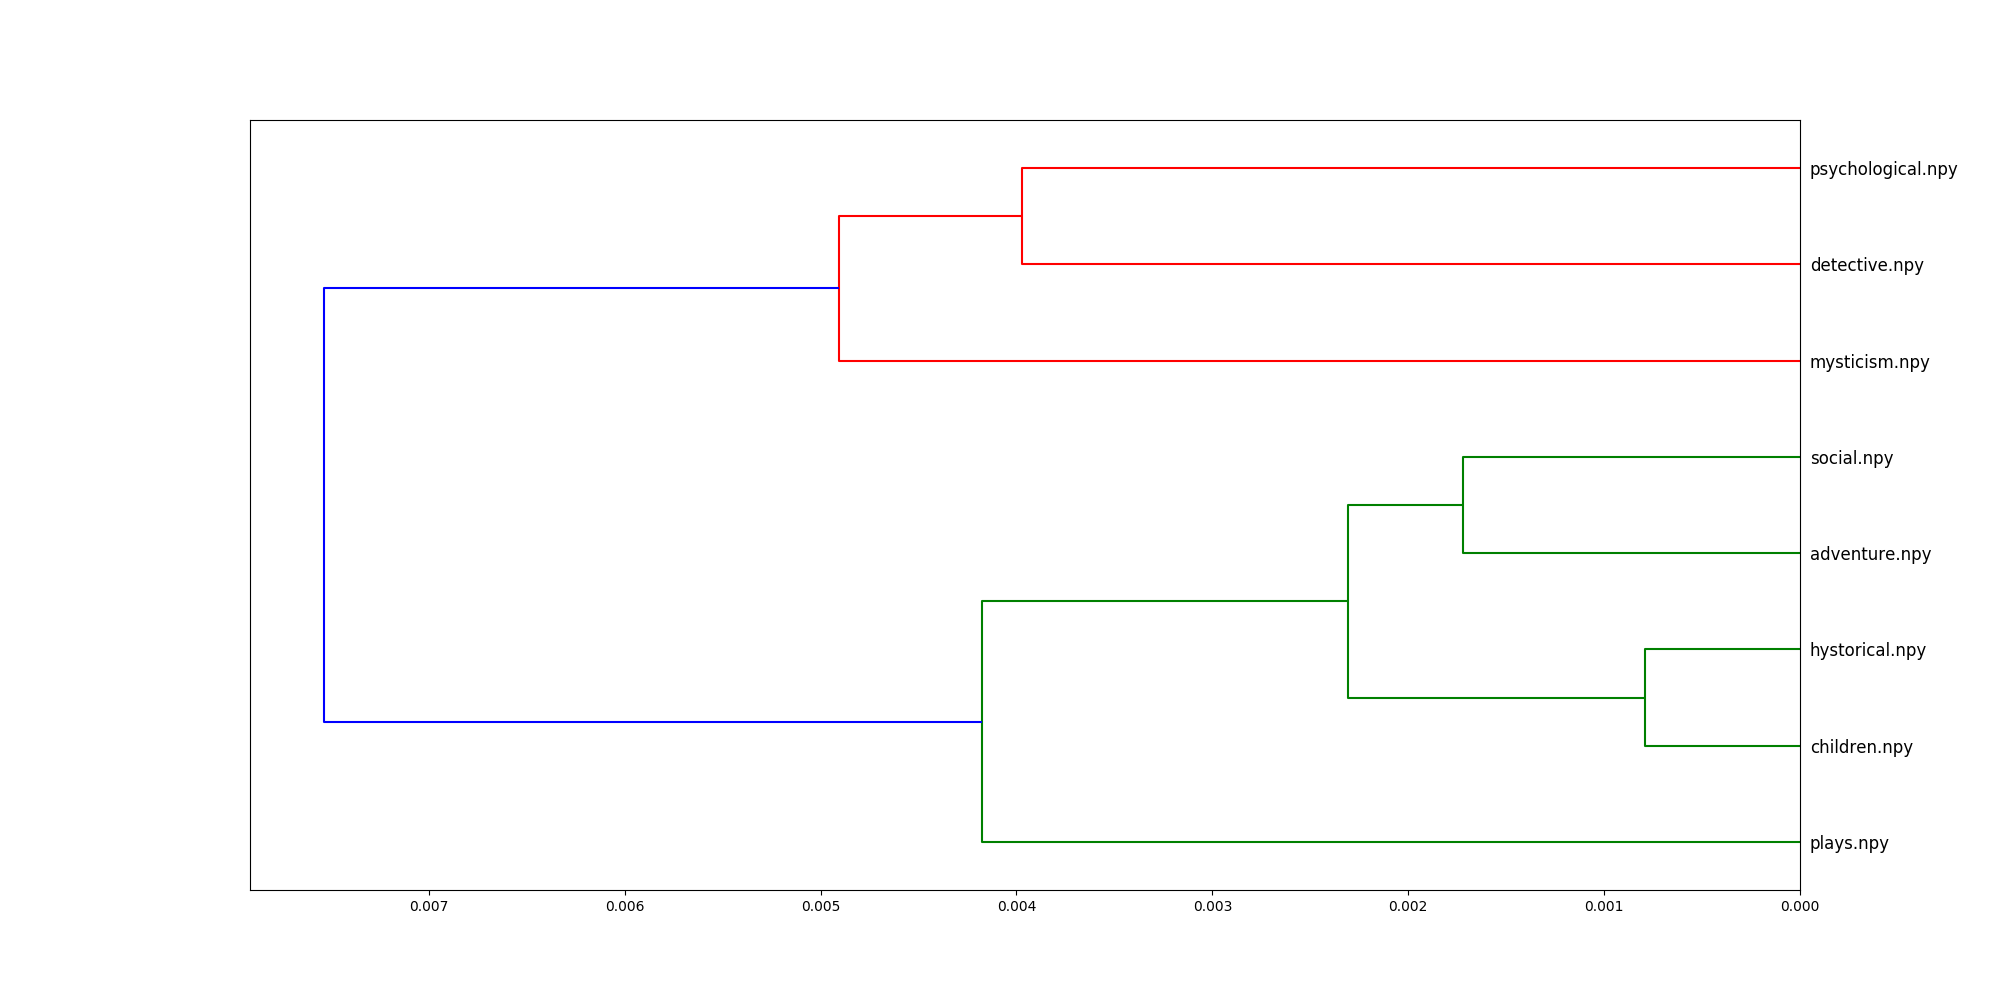
\includegraphics[width=\textwidth]{figures/stopwords_excluded/dendrogram_d0.png}
			\caption{No stop words, $d = 0$}
			\label{fig:sw:d0}
		\end{subfigure}\hfill
		\\
		\begin{subfigure}[t]{0.475\textwidth}
			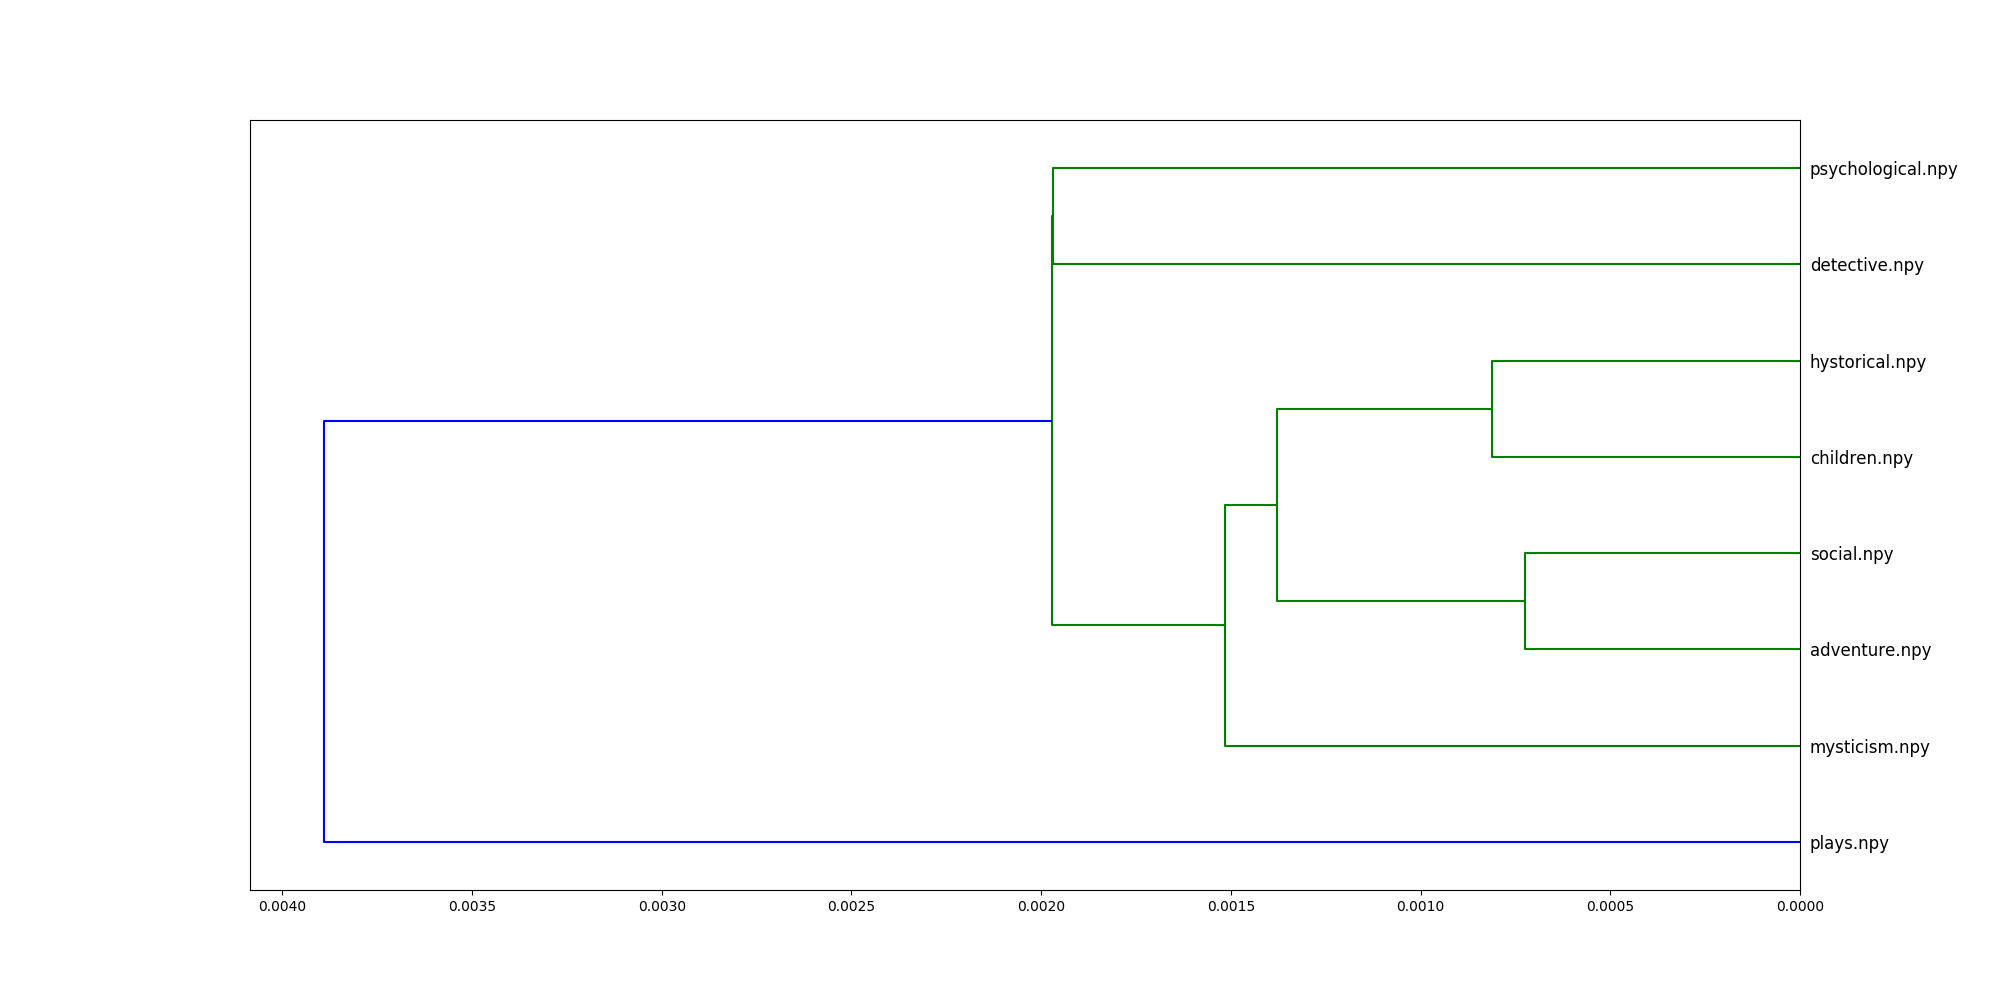
\includegraphics[width=\textwidth]{figures/all_words/dendrogram_d1.png}
			\caption{All words, $d =1$}
			\label{fig:all:d1}
		\end{subfigure}\hfill
		\begin{subfigure}[t]{0.475\textwidth}
			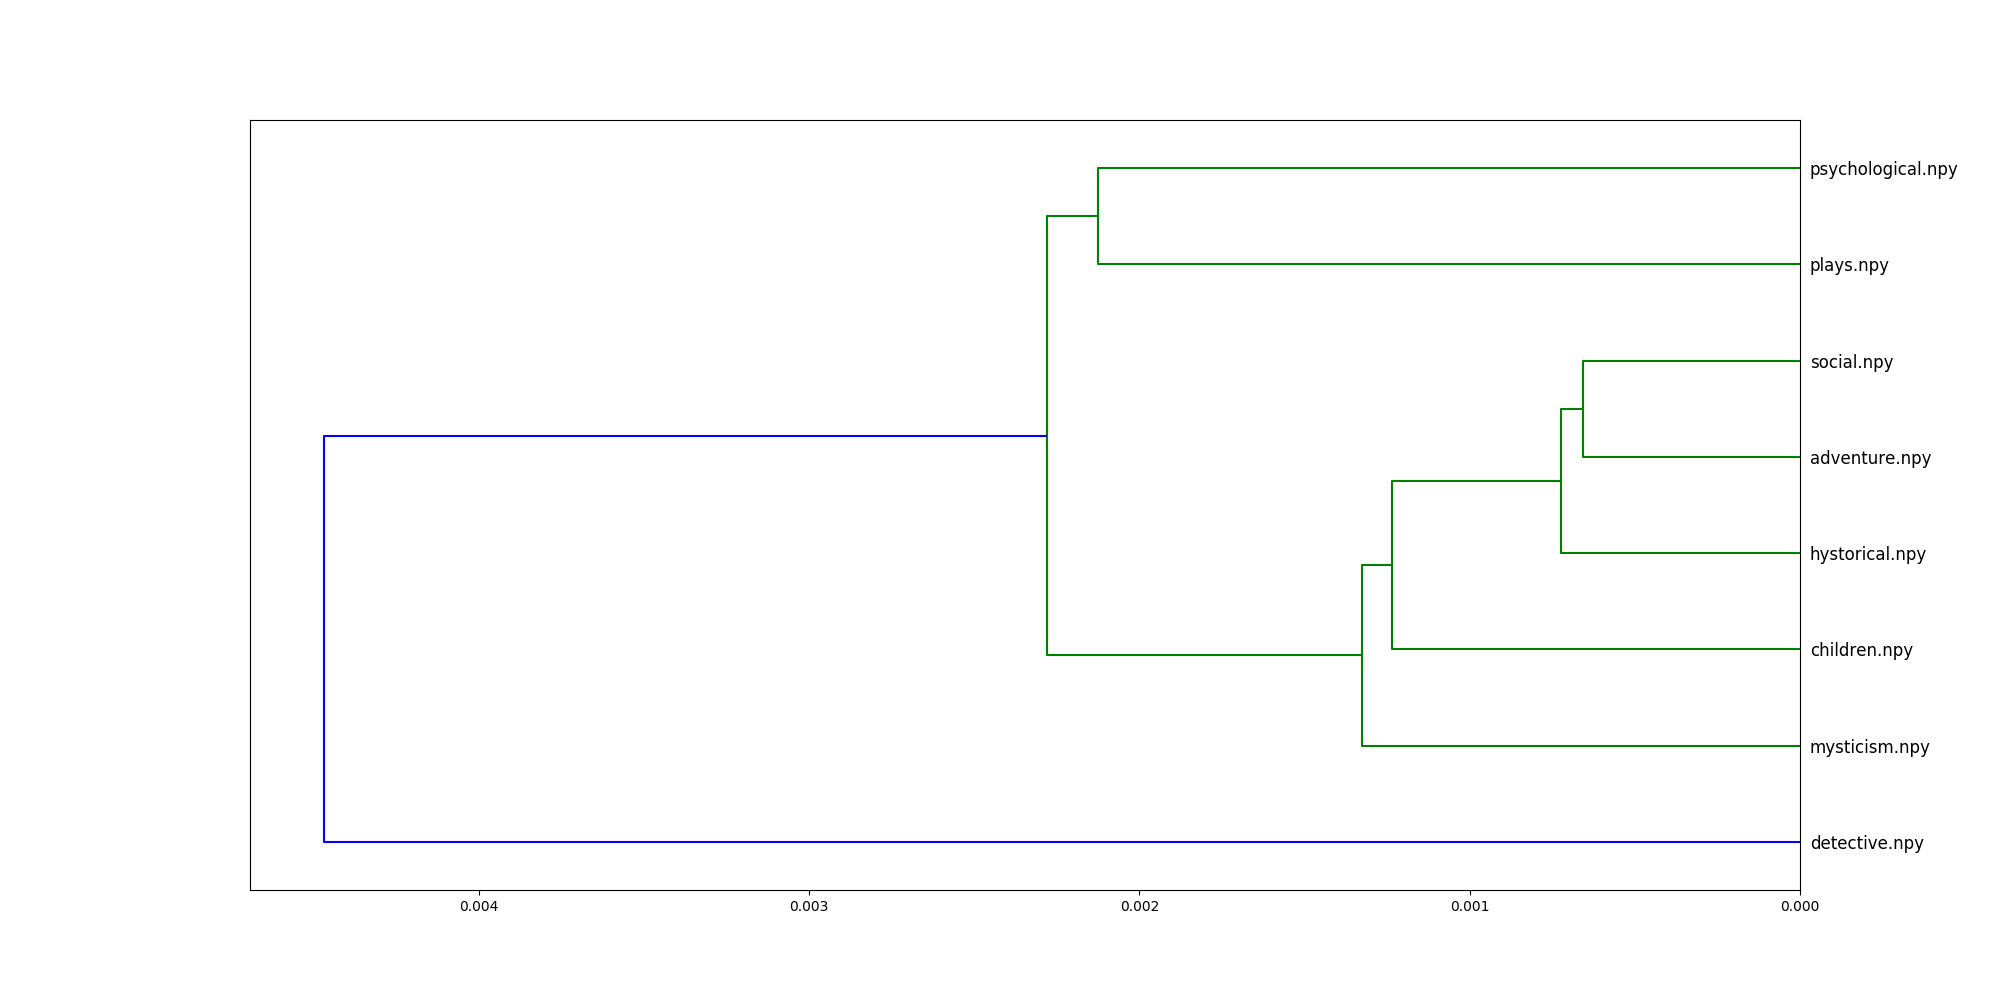
\includegraphics[width=\textwidth]{figures/stopwords_excluded/dendrogram_d1.png}
			\caption{No stop words, $d = 1$}
			\label{fig:sw:d1}
		\end{subfigure}\hfill
		\\
		\begin{subfigure}[t]{0.475\textwidth}
			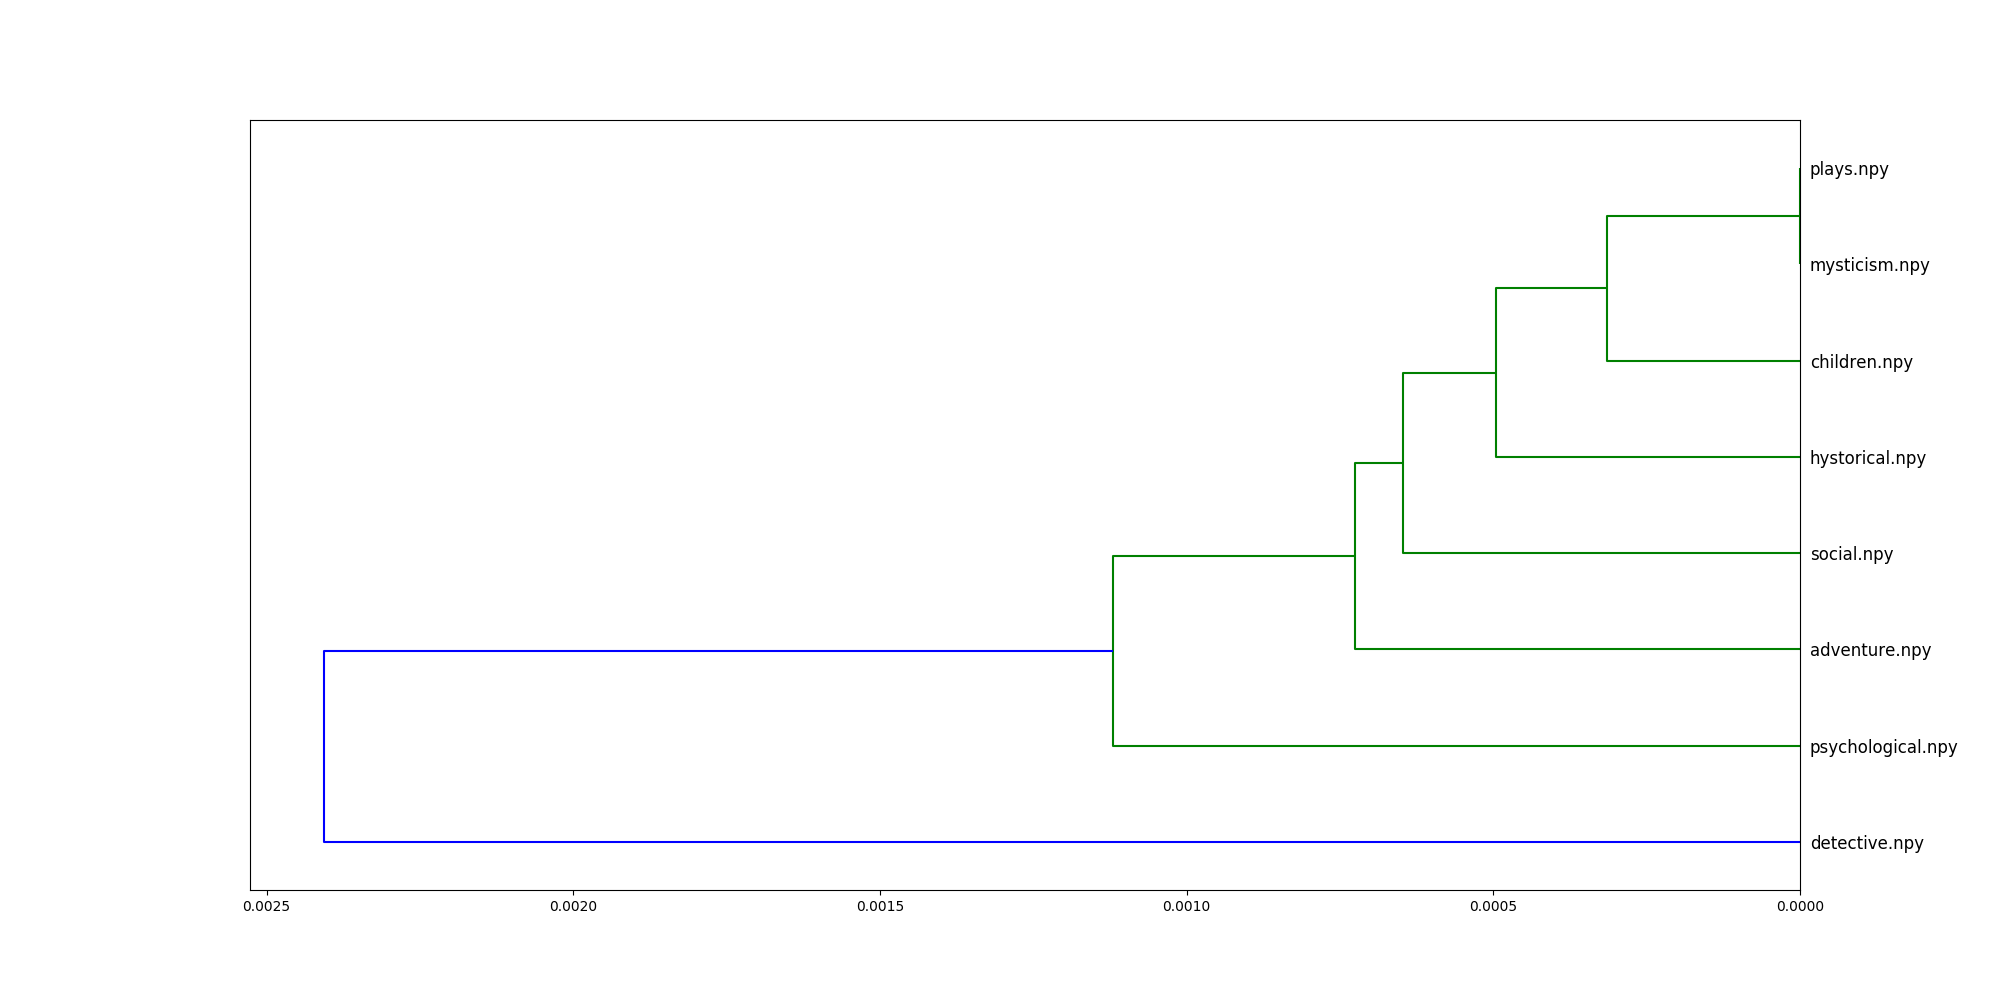
\includegraphics[width=\textwidth]{figures/all_words/dendrogram_d2.png}
			\caption{All words, $d = 2$}
			\label{fig:all:d2}
		\end{subfigure}\hfill
		\begin{subfigure}[t]{0.475\textwidth}
			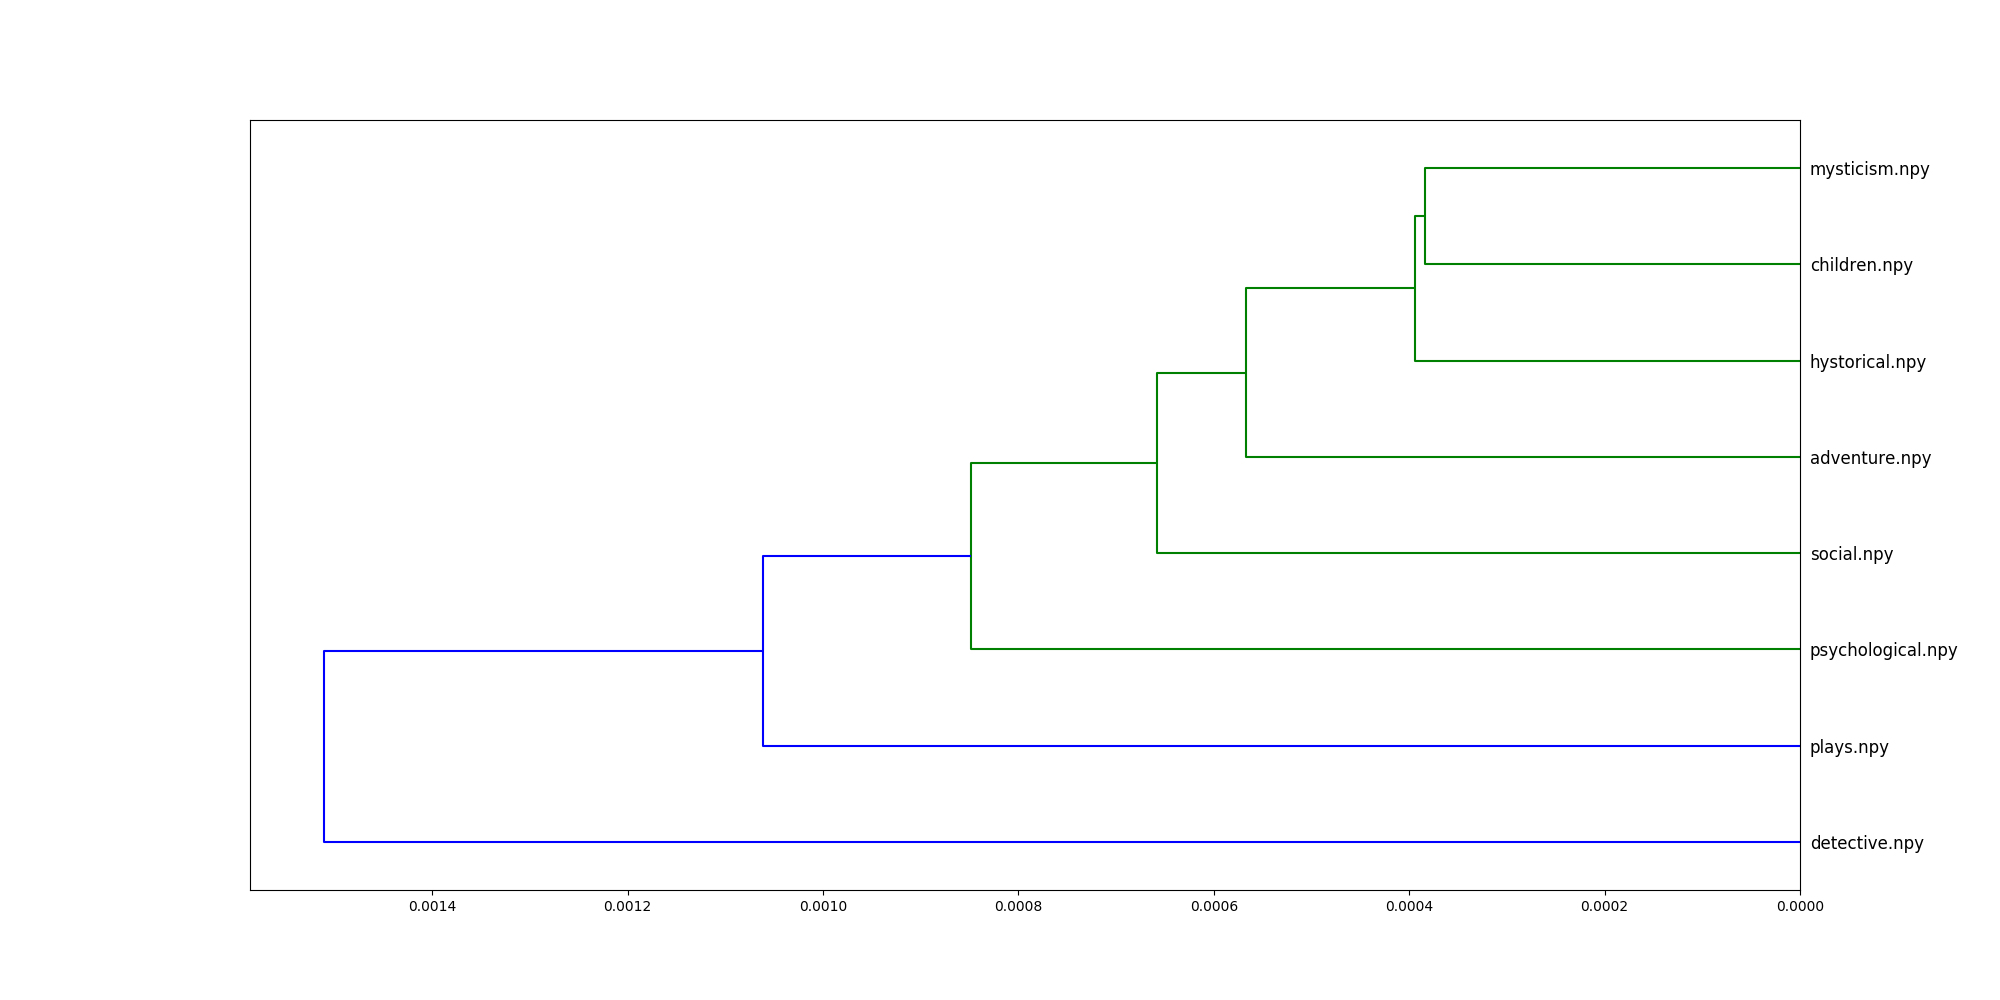
\includegraphics[width=\textwidth]{figures/stopwords_excluded/dendrogram_d2.png}
			\caption{No stop words, $d = 2$}
			\label{fig:sw:d2}
		\end{subfigure}\hfill
		\caption{Agglomerative clustering based on the bottleneck distance between all categories. On the left we have included all words, whilst on the right we omitted the stop words. Each row presents a single dimension.}
		\label{fig:dendro}
	\end{figure}
	
	\bibliographystyle{elsarticle-num}
	\bibliography{bibliography}
	
\end{document}
